\documentclass[aspectratio=169,10pt]{beamer}

\usepackage[T1]{fontenc}
\usepackage[utf8]{inputenc}
\usepackage{lmodern}
\usepackage{amsmath,amssymb,bm}
\usepackage{graphicx}
\usepackage{tikz}
\usepackage{booktabs}
\usepackage{hyperref}
\usetikzlibrary{arrows.meta,positioning,calc,shapes.geometric}

\definecolor{URBlue}{RGB}{0,56,101}
\definecolor{URGold}{RGB}{204,153,0}
\definecolor{RwandaGreen}{RGB}{0,126,94}
\definecolor{DeepInk}{RGB}{18,33,58}
\definecolor{SoftBlue}{RGB}{232,241,249}
\definecolor{SoftGold}{RGB}{255,247,224}
\definecolor{AlertRed}{RGB}{184,69,69}
\definecolor{Muted}{RGB}{83,94,108}

\newcommand{\Rzero}{\mathcal{R}_0}
\newcommand{\CaputoD}[2]{{}^{C}D_{#1}^{#2}}
\newcommand{\beff}{\beta_{\mathrm{eff}}}
\newcommand{\taueff}{\tau_{\mathrm{eff}}}
\newcommand{\rhoeff}{\rho_{\mathrm{eff}}}
\newcommand{\appurl}{https://hiv-model.onrender.com/}

\setbeamertemplate{navigation symbols}{}
\setbeamertemplate{itemize item}{\color{RwandaGreen}\raisebox{0.2ex}{\scriptsize$\blacktriangleright$}}
\setbeamertemplate{itemize subitem}{\color{URGold}\tiny$\bullet$}
\setbeamercolor{normal text}{fg=DeepInk,bg=white}
\setbeamercolor{frametitle}{fg=DeepInk,bg=white}
\setbeamercolor{title}{fg=white}
\setbeamerfont{frametitle}{series=\bfseries,size=\Large}
\setbeamerfont{title}{series=\bfseries,size=\huge}
\setbeamerfont{subtitle}{size=\large}

\setbeamertemplate{frametitle}{
  \vspace{0.35cm}
  \begin{beamercolorbox}[wd=\paperwidth,leftskip=0.55cm,rightskip=0.55cm]{frametitle}
    \insertframetitle
    \ifx\insertframesubtitle\empty\else
      \par{\small\color{Muted}\insertframesubtitle}
    \fi
  \end{beamercolorbox}
  \vspace{-0.1cm}
  \hspace{0.55cm}{\color{URGold}\rule{2.2cm}{1.4pt}}{\color{RwandaGreen}\rule{8.3cm}{1.4pt}}
}

\setbeamertemplate{footline}{
  \leavevmode
  \hbox{
    \begin{beamercolorbox}[wd=.72\paperwidth,ht=2.8ex,dp=1.1ex,leftskip=0.55cm]{normal text}
      {\scriptsize FracHIV-SITA Lab \hspace{0.4em}|\hspace{0.4em} Dashboard-focused thesis presentation}
    \end{beamercolorbox}
    \begin{beamercolorbox}[wd=.28\paperwidth,ht=2.8ex,dp=1.1ex,rightskip=0.55cm plus 1fil]{normal text}
      \hfill{\scriptsize \insertframenumber/10}
    \end{beamercolorbox}
  }
}

\newcommand{\sectiontag}[1]{%
  {\small\bfseries\color{URGold}#1}\par\vspace{0.15cm}
}

\newcommand{\metriccard}[3]{%
  \begin{tikzpicture}
    \node[
      fill=#1,
      text=white,
      rounded corners=3pt,
      minimum width=3.15cm,
      minimum height=1.55cm,
      inner sep=6pt,
      align=left
    ] {
      {\scriptsize\bfseries #2}\\[2pt]
      {\Large\bfseries #3}
    };
  \end{tikzpicture}
}

\newcommand{\softbox}[2]{%
  \begin{tikzpicture}
    \node[
      fill=#1,
      draw=#1!70!black,
      rounded corners=3pt,
      inner sep=8pt,
      text width=\linewidth-0.45cm,
      align=left
    ] {#2};
  \end{tikzpicture}
}

\title{Fractional-Order HIV SITA Dashboard}
\subtitle{Social Behaviour Interventions, Memory Effects, and Live Simulation Evidence}
\author{NDACYAYISABA Lambert}
\institute{University of Rwanda -- College of Science and Technology\\Supervisor: Dr. MUHIRWA Jean Pierre}
\date{Kigali, Rwanda}

\begin{document}

% 1
\begin{frame}[plain]
  \begin{tikzpicture}[remember picture,overlay]
    \fill[DeepInk] (current page.south west) rectangle (current page.north east);
    \fill[URBlue] (current page.south west) rectangle ($(current page.north east)+(0,-6.8)$);
    \fill[RwandaGreen] ($(current page.south west)+(0,0)$) rectangle ($(current page.south east)+(0,0.55)$);
    \fill[URGold] ($(current page.south west)+(0,0.55)$) rectangle ($(current page.south east)+(0,0.72)$);
    \node[opacity=0.16,anchor=south east] at ($(current page.south east)+(-0.1,0.65)$)
      {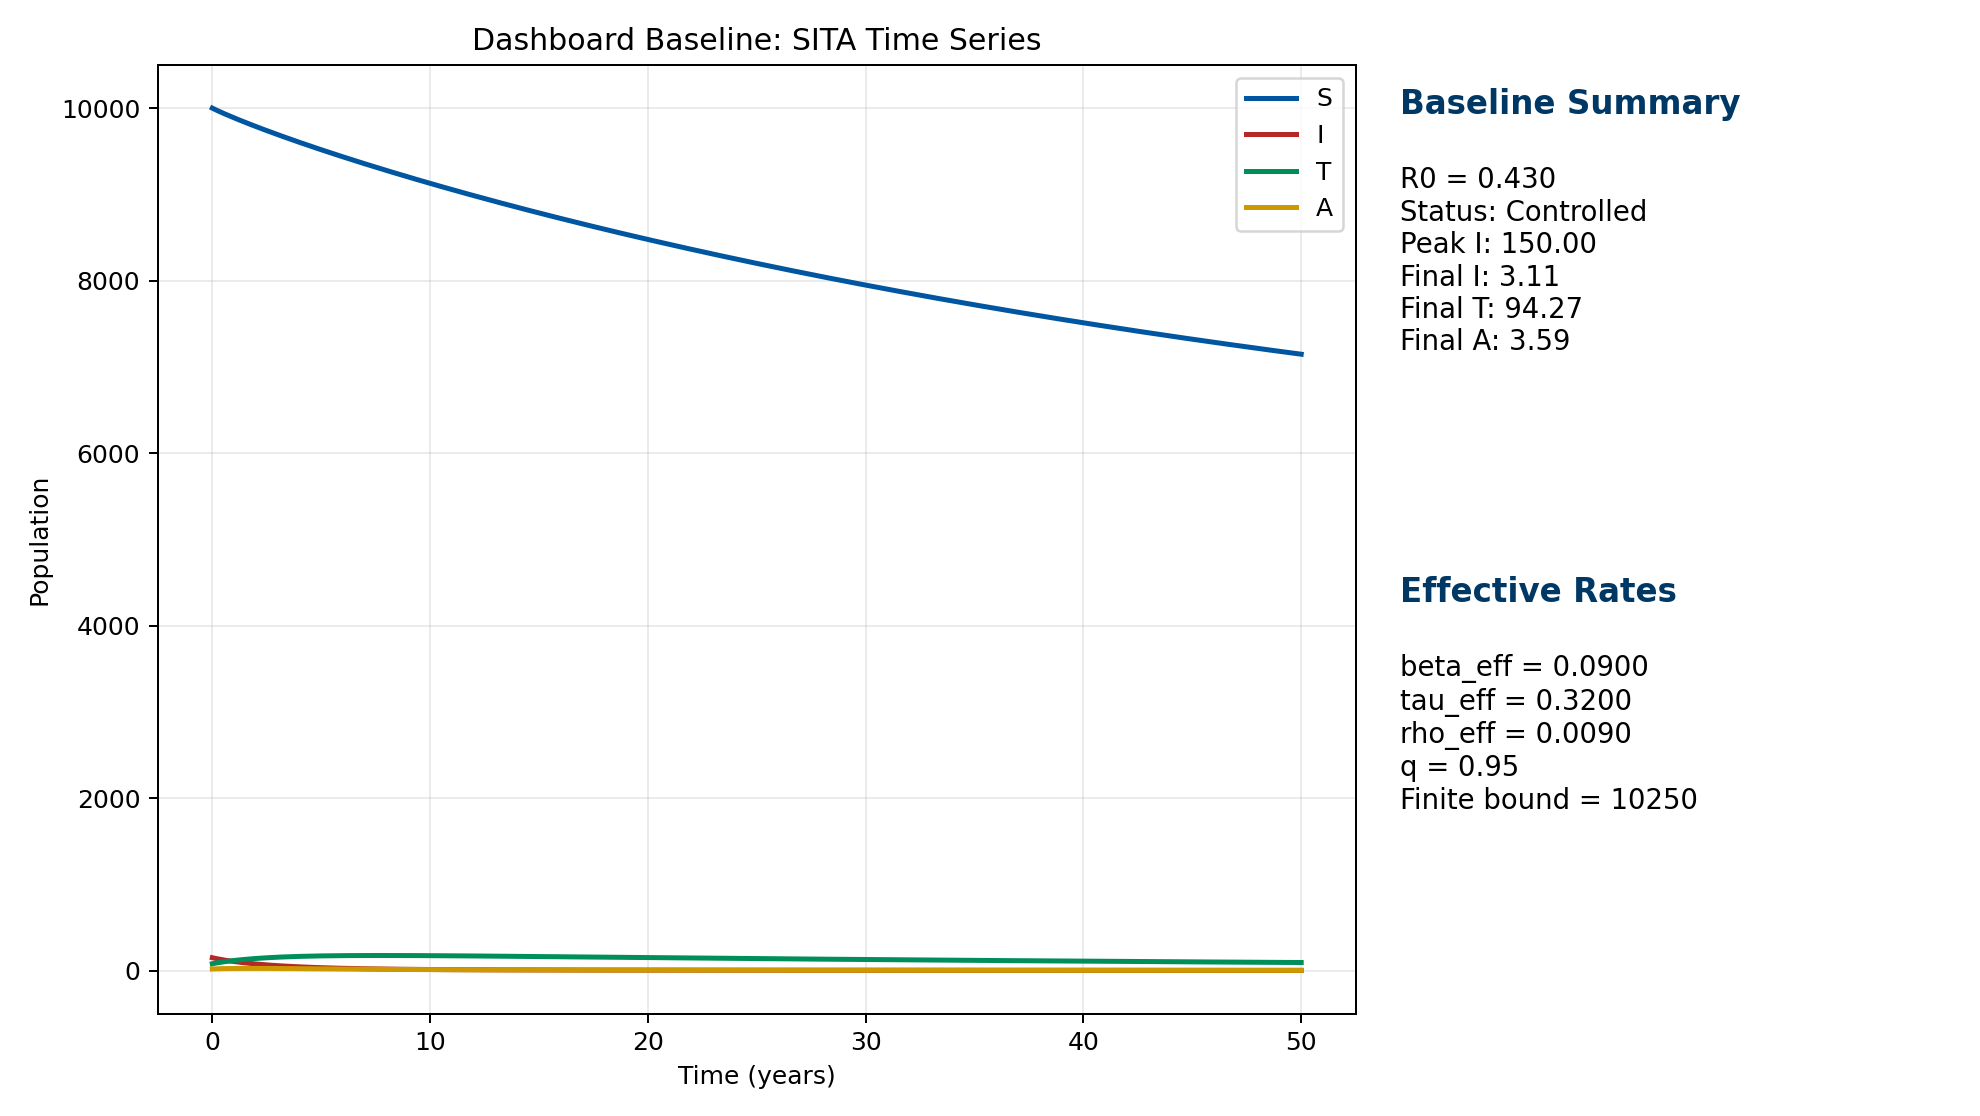
\includegraphics[width=0.67\paperwidth]{../thesis/dashboardBaselineFigure.png}};
    \node[anchor=north west] at ($(current page.north west)+(0.65,-0.55)$)
      {
\includegraphics[width=1.22cm]{../thesis/logo.png}};
    \node[anchor=north east,align=right,text=white] at ($(current page.north east)+(-0.65,-0.7)$)
      {\small University of Rwanda\\\small Kigali, Rwanda};
    \node[anchor=west,align=left,text=white] at ($(current page.west)+(0.72,0.82)$)
      {{\fontsize{25}{29}\selectfont\bfseries Fractional-Order HIV}\\[3pt]
       {\fontsize{25}{29}\selectfont\bfseries SITA Dashboard}\\[7pt]
       {\large Social behaviour interventions, memory effects, and live simulation}\\[14pt]
       {\normalsize\bfseries NDACYAYISABA Lambert}\\[2pt]
       {\small Supervisor: Dr. MUHIRWA Jean Pierre}};
    \node[anchor=south west,align=left,text=white] at ($(current page.south west)+(0.72,0.98)$)
      {\small Live dashboard: \texttt{\appurl}};
  \end{tikzpicture}
\end{frame}

% 2
\begin{frame}{Background / Motivation}
  \begin{columns}[T,onlytextwidth]
    \begin{column}{0.56\textwidth}
      \sectiontag{Why this topic matters}
      \begin{itemize}
        \item HIV/AIDS remains shaped by biological, behavioural, and social factors.
        \item Rwanda has made strong progress in testing, treatment, and viral suppression, but prevention and adherence remain important.
        \item Public-health behaviour has memory: awareness, stigma reduction, testing history, and adherence patterns can influence future dynamics.
      \end{itemize}
      \vspace{0.25cm}
      \softbox{SoftBlue}{\textbf{Presentation focus:} the dashboard makes the mathematical model visible, testable, and easier to defend through live simulation.}
    \end{column}
    \begin{column}{0.39\textwidth}
      \vspace{0.15cm}
      \metriccard{URBlue}{Rwanda context}{HIV prevention}
      \vspace{0.18cm}
      \metriccard{RwandaGreen}{Mathematical lens}{Fractional memory}
      \vspace{0.18cm}
      \metriccard{URGold}{Output}{Interactive dashboard}
    \end{column}
  \end{columns}
\end{frame}

% 3
\begin{frame}{Problem Statement}
  \begin{columns}[T,onlytextwidth]
    \begin{column}{0.47\textwidth}
      \sectiontag{Gap}
      \begin{itemize}
        \item Ordinary HIV models often depend only on the present state.
        \item Social behaviour is frequently treated as fixed or simplified.
        \item Many mathematical reports stop at equations and static graphs.
      \end{itemize}
    \end{column}
    \begin{column}{0.47\textwidth}
      \sectiontag{This project responds by}
      \begin{itemize}
        \item Formulating a fractional-order SITA model.
        \item Adding bounded social behaviour interventions.
        \item Building a working dashboard for simulation, scenario comparison, sensitivity analysis, and exports.
      \end{itemize}
    \end{column}
  \end{columns}
  \vspace{0.45cm}
  \softbox{SoftGold}{\textbf{Central question:} How do fractional memory and social behaviour interventions affect simulated HIV dynamics in a Rwanda-aware academic dashboard?}
\end{frame}

% 4
\begin{frame}{Objectives}
  \begin{columns}[T,onlytextwidth]
    \begin{column}{0.58\textwidth}
      \sectiontag{Main objective}
      To formulate, analyse, and computationally simulate a fractional-order SITA model of HIV transmission incorporating social behaviour interventions.
      \vspace{0.35cm}
      \sectiontag{Specific objectives}
      \begin{itemize}
        \item Construct the SITA model with Caputo fractional derivative.
        \item Derive the disease-free equilibrium and reproduction number.
        \item Analyse positivity, boundedness, and threshold behaviour.
        \item Implement a numerical ABM-type solver and dashboard.
        \item Compare intervention scenarios, memory effects, and sensitivity indices.
      \end{itemize}
    \end{column}
    \begin{column}{0.37\textwidth}
      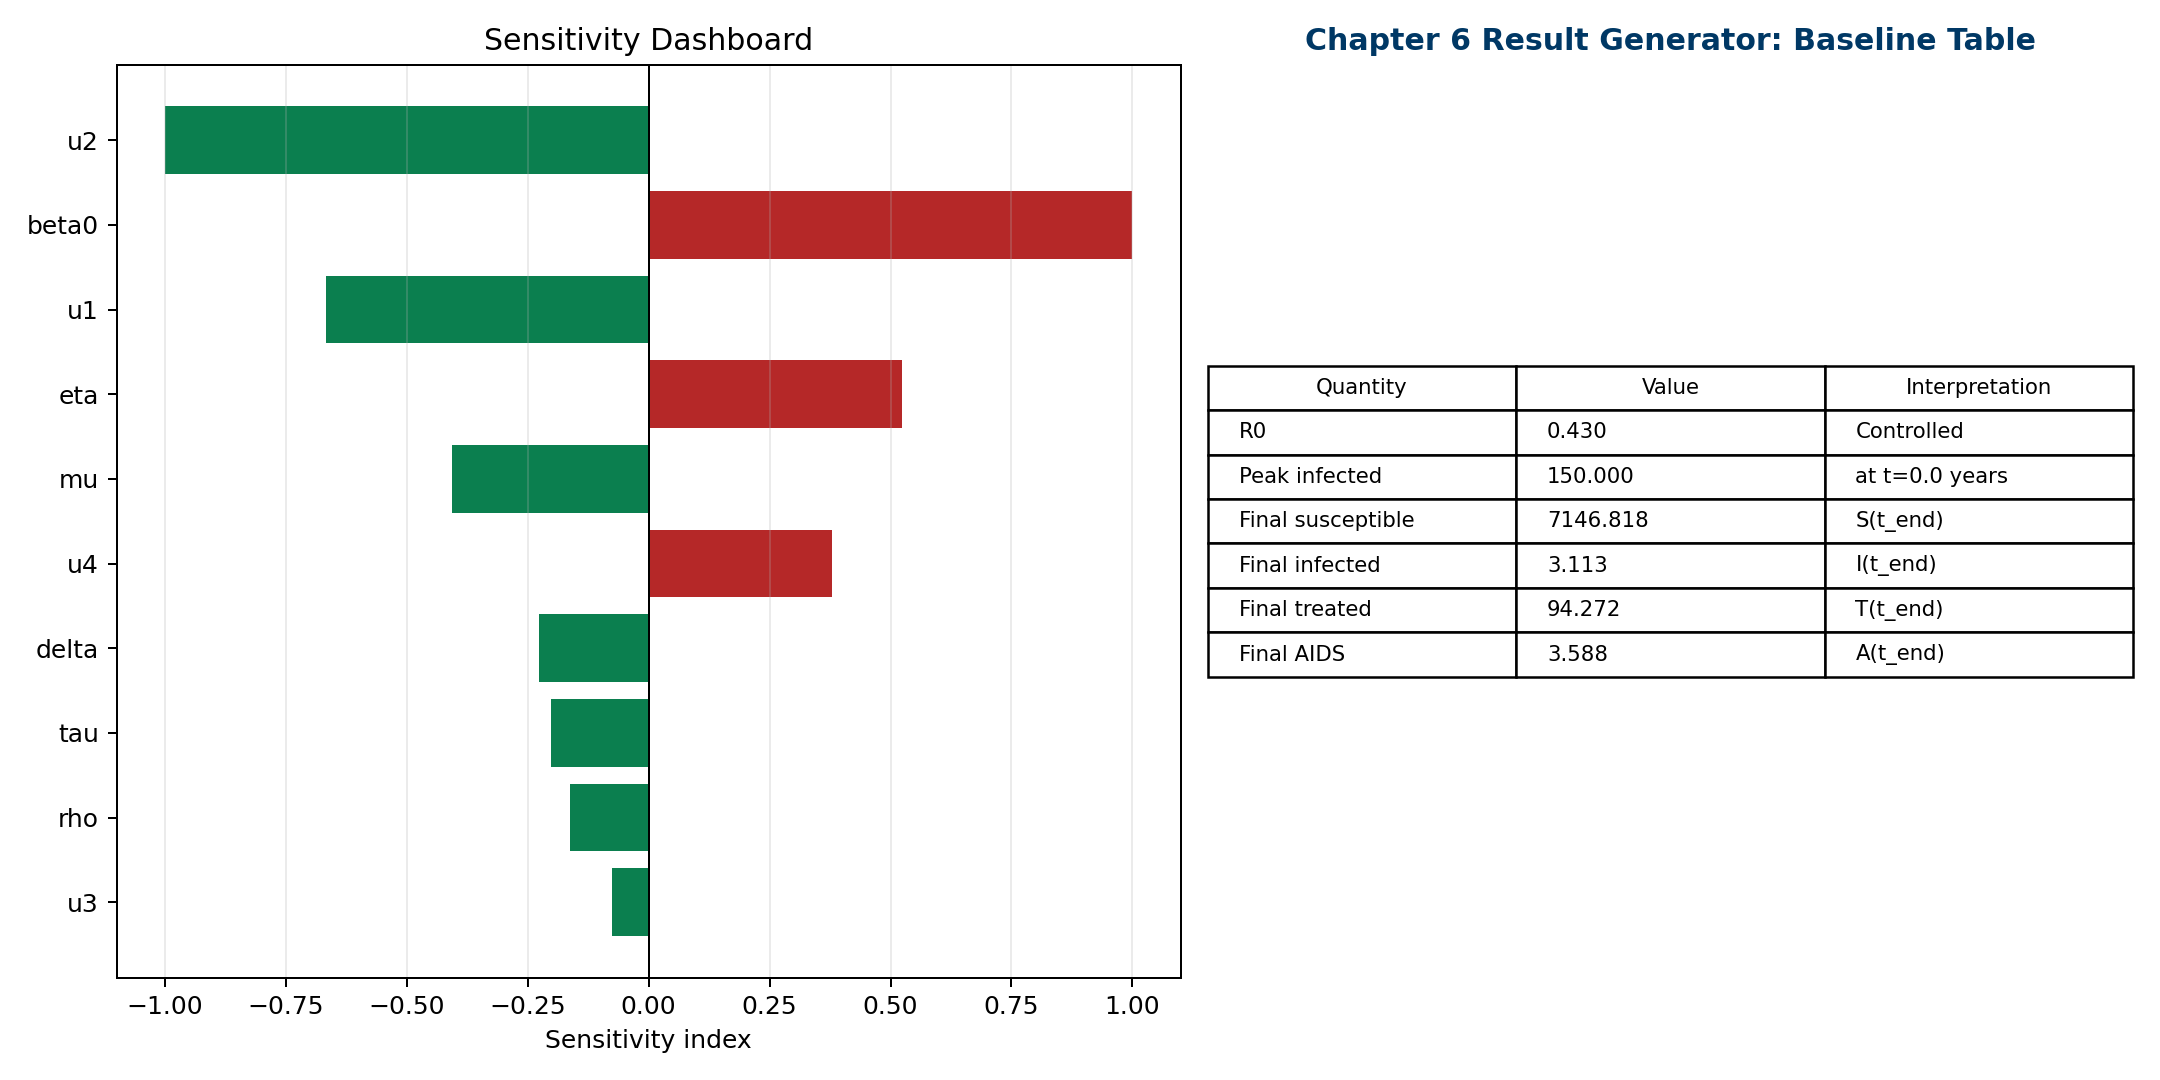
\includegraphics[width=0.92\linewidth]{../thesis/dashboardSensitivityChapter6Figure.png}
      \vspace{0.2cm}
      {\scriptsize\color{Muted}Dashboard evidence is the central presentation artifact.}
    \end{column}
  \end{columns}
\end{frame}

% 5
\begin{frame}{Model Diagram: SITA}
  \begin{center}
  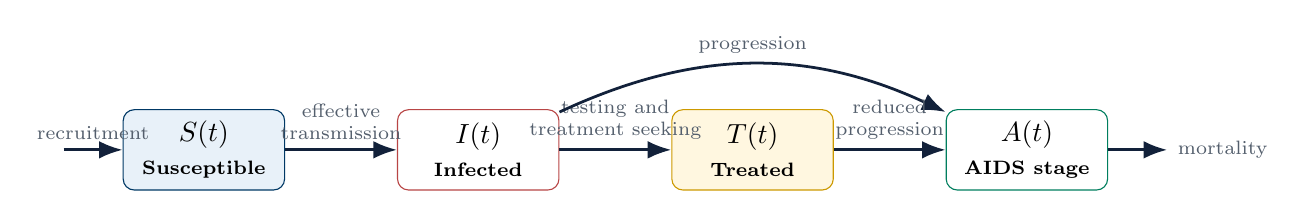
\begin{tikzpicture}[
    node distance=1.42cm,
    comp/.style={draw,rounded corners=4pt,minimum width=2.05cm,minimum height=1.02cm,align=center,font=\bfseries},
    arrow/.style={-{Latex[length=3mm]},line width=1pt,DeepInk},
    lab/.style={font=\scriptsize,align=center,Muted}
  ]
    \node[comp,fill=SoftBlue,draw=URBlue] (S) {$S(t)$\\{\scriptsize Susceptible}};
    \node[comp,fill=white,draw=AlertRed,right=of S] (I) {$I(t)$\\{\scriptsize Infected}};
    \node[comp,fill=SoftGold,draw=URGold,right=of I] (T) {$T(t)$\\{\scriptsize Treated}};
    \node[comp,fill=white,draw=RwandaGreen,right=of T] (A) {$A(t)$\\{\scriptsize AIDS stage}};

    \draw[arrow] (S) -- node[lab,above] {effective\\transmission} (I);
    \draw[arrow] (I) -- node[lab,above] {testing and\\treatment seeking} (T);
    \draw[arrow] (I) to[bend left=25] node[lab,above] {progression} (A);
    \draw[arrow] (T) -- node[lab,above] {reduced\\progression} (A);
    \draw[arrow] ($(S.west)+(-0.75,0)$) -- node[lab,above] {recruitment} (S);
    \draw[arrow] (A) -- ($(A.east)+(0.75,0)$) node[lab,right] {mortality};
  \end{tikzpicture}
  \end{center}
  \vspace{0.25cm}
  \begin{columns}[T,onlytextwidth]
    \begin{column}{0.5\textwidth}
      \softbox{SoftBlue}{\textbf{Intervention effects:} $u_1$ awareness, $u_2$ safer behaviour, $u_3$ testing, $u_4$ adherence.}
    \end{column}
    \begin{column}{0.45\textwidth}
      \softbox{SoftGold}{\textbf{Dashboard role:} each slider changes the effective rates before running the simulation.}
    \end{column}
  \end{columns}
\end{frame}

% 6
\begin{frame}{Fractional-Order Model}
  \begin{columns}[T,onlytextwidth]
    \begin{column}{0.58\textwidth}
      \sectiontag{Caputo fractional dynamics}
      \[
        \CaputoD{t}{q}X(t)=F(t,X(t)),\qquad 0<q\leq1
      \]
      \[
      \begin{aligned}
        \CaputoD{t}{q}S &= \Lambda-\beff S(I+\eta T)-\mu S,\\
        \CaputoD{t}{q}I &= \beff S(I+\eta T)-(\taueff+\delta+\mu)I,\\
        \CaputoD{t}{q}T &= \taueff I-(\rhoeff+\mu)T,\\
        \CaputoD{t}{q}A &= \delta I+\rhoeff T-(d+\mu)A.
      \end{aligned}
      \]
    \end{column}
    \begin{column}{0.37\textwidth}
      \sectiontag{Intervention-adjusted rates}
      \[
        \beff=\beta_0(1-u_1)(1-u_2)
      \]
      \[
        \taueff=\tau(1+u_3),\qquad
        \rhoeff=\rho(1-u_4)
      \]
      \vspace{0.2cm}
      \softbox{SoftBlue}{When $q=1$, the model becomes ordinary. When $q<1$, the model carries memory of past states.}
    \end{column}
  \end{columns}
\end{frame}

% 7
\begin{frame}{Numerical Scheme + Dashboard}
  \begin{columns}[T,onlytextwidth]
    \begin{column}{0.43\textwidth}
      \sectiontag{Computational implementation}
      \begin{itemize}
        \item ABM-type predictor-corrector solver for Caputo fractional equations.
        \item Real-time dashboard controls for parameters, initial conditions, intervention levels, and simulation horizon.
        \item Automatic outputs: trajectories, $\Rzero$, scenario tables, memory comparison, sensitivity ranking, and exports.
      \end{itemize}
      \vspace{0.2cm}
      \softbox{SoftGold}{\textbf{Live system:} \texttt{\appurl}}
    \end{column}
    \begin{column}{0.53\textwidth}
      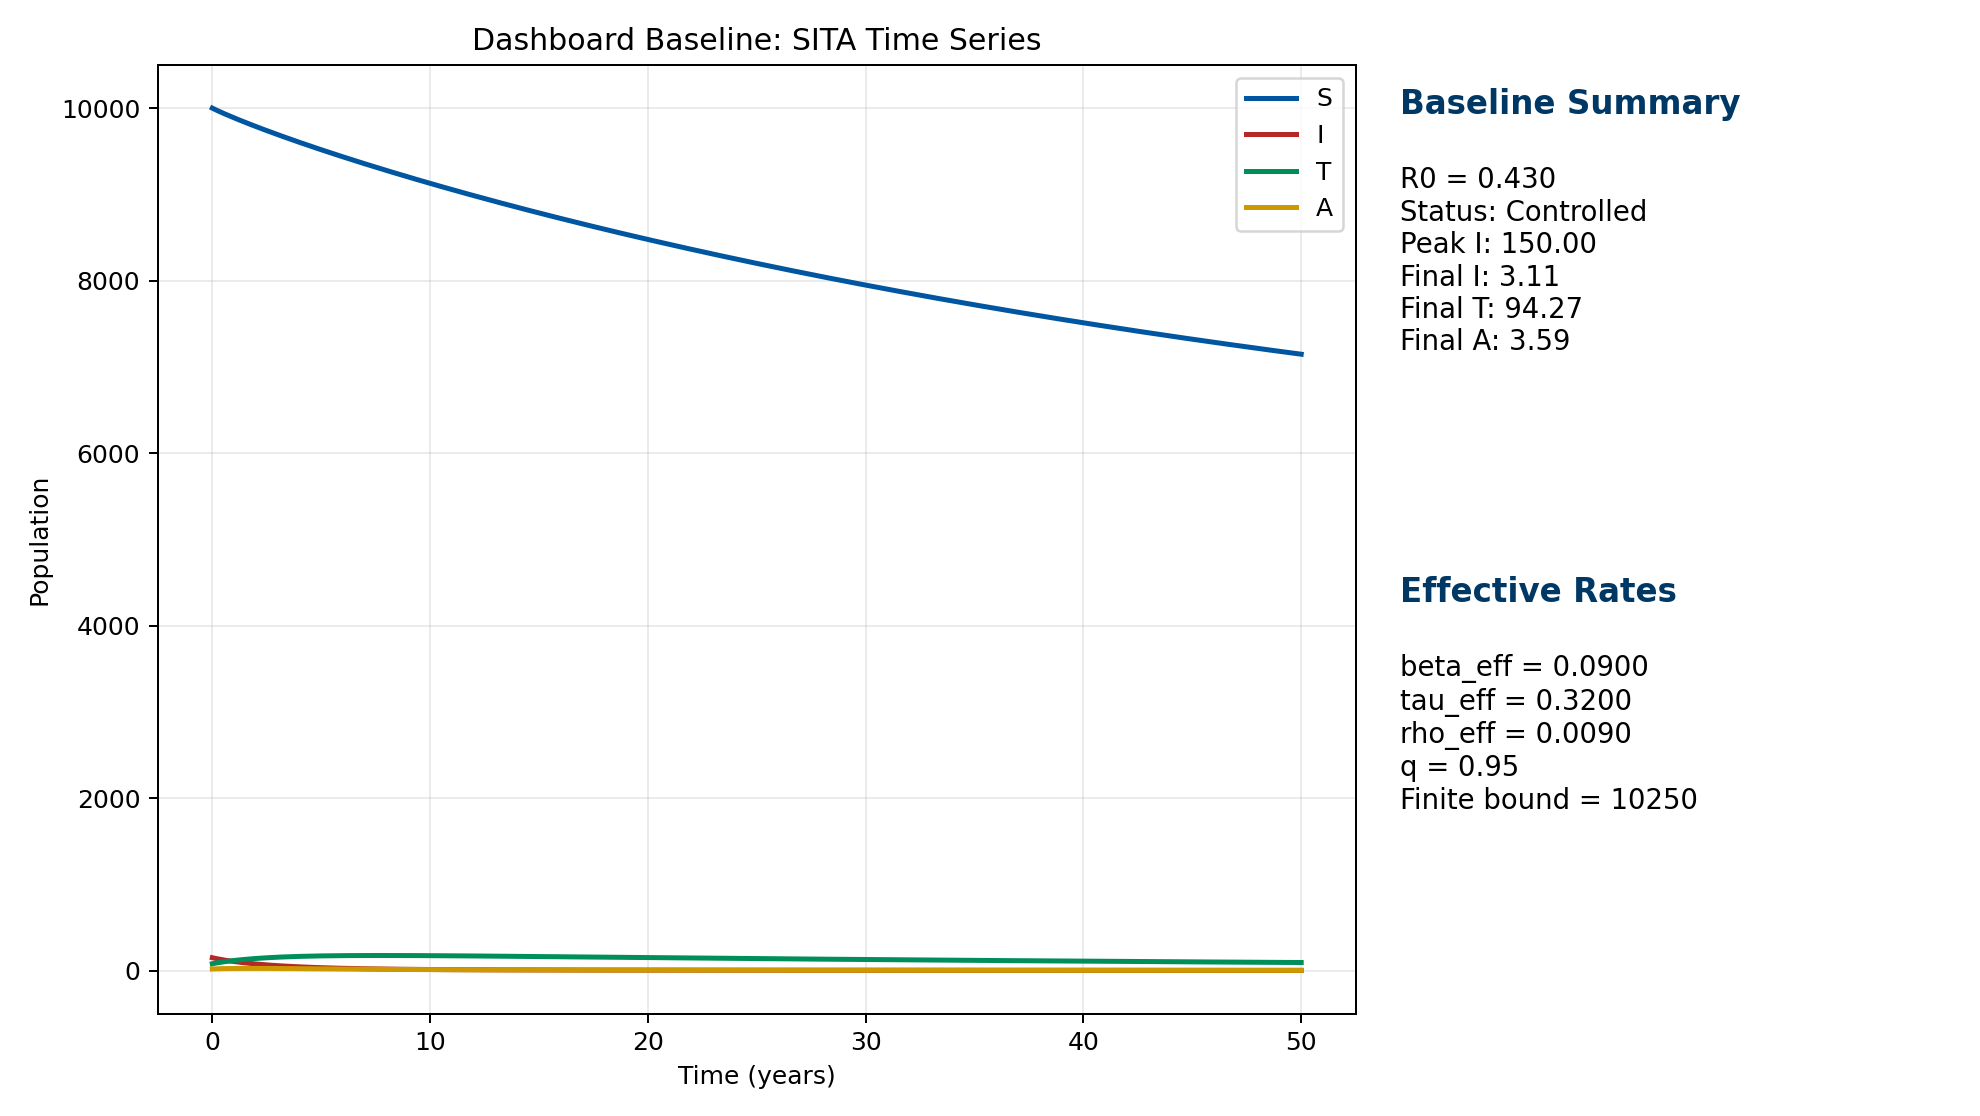
\includegraphics[width=0.96\linewidth]{../thesis/dashboardBaselineFigure.png}
      \vspace{0.08cm}
      {\scriptsize\color{Muted}Dashboard baseline trajectory view.}
    \end{column}
  \end{columns}
\end{frame}

% 8
\begin{frame}{Simulation Results}
  \begin{columns}[T,onlytextwidth]
    \begin{column}{0.49\textwidth}
      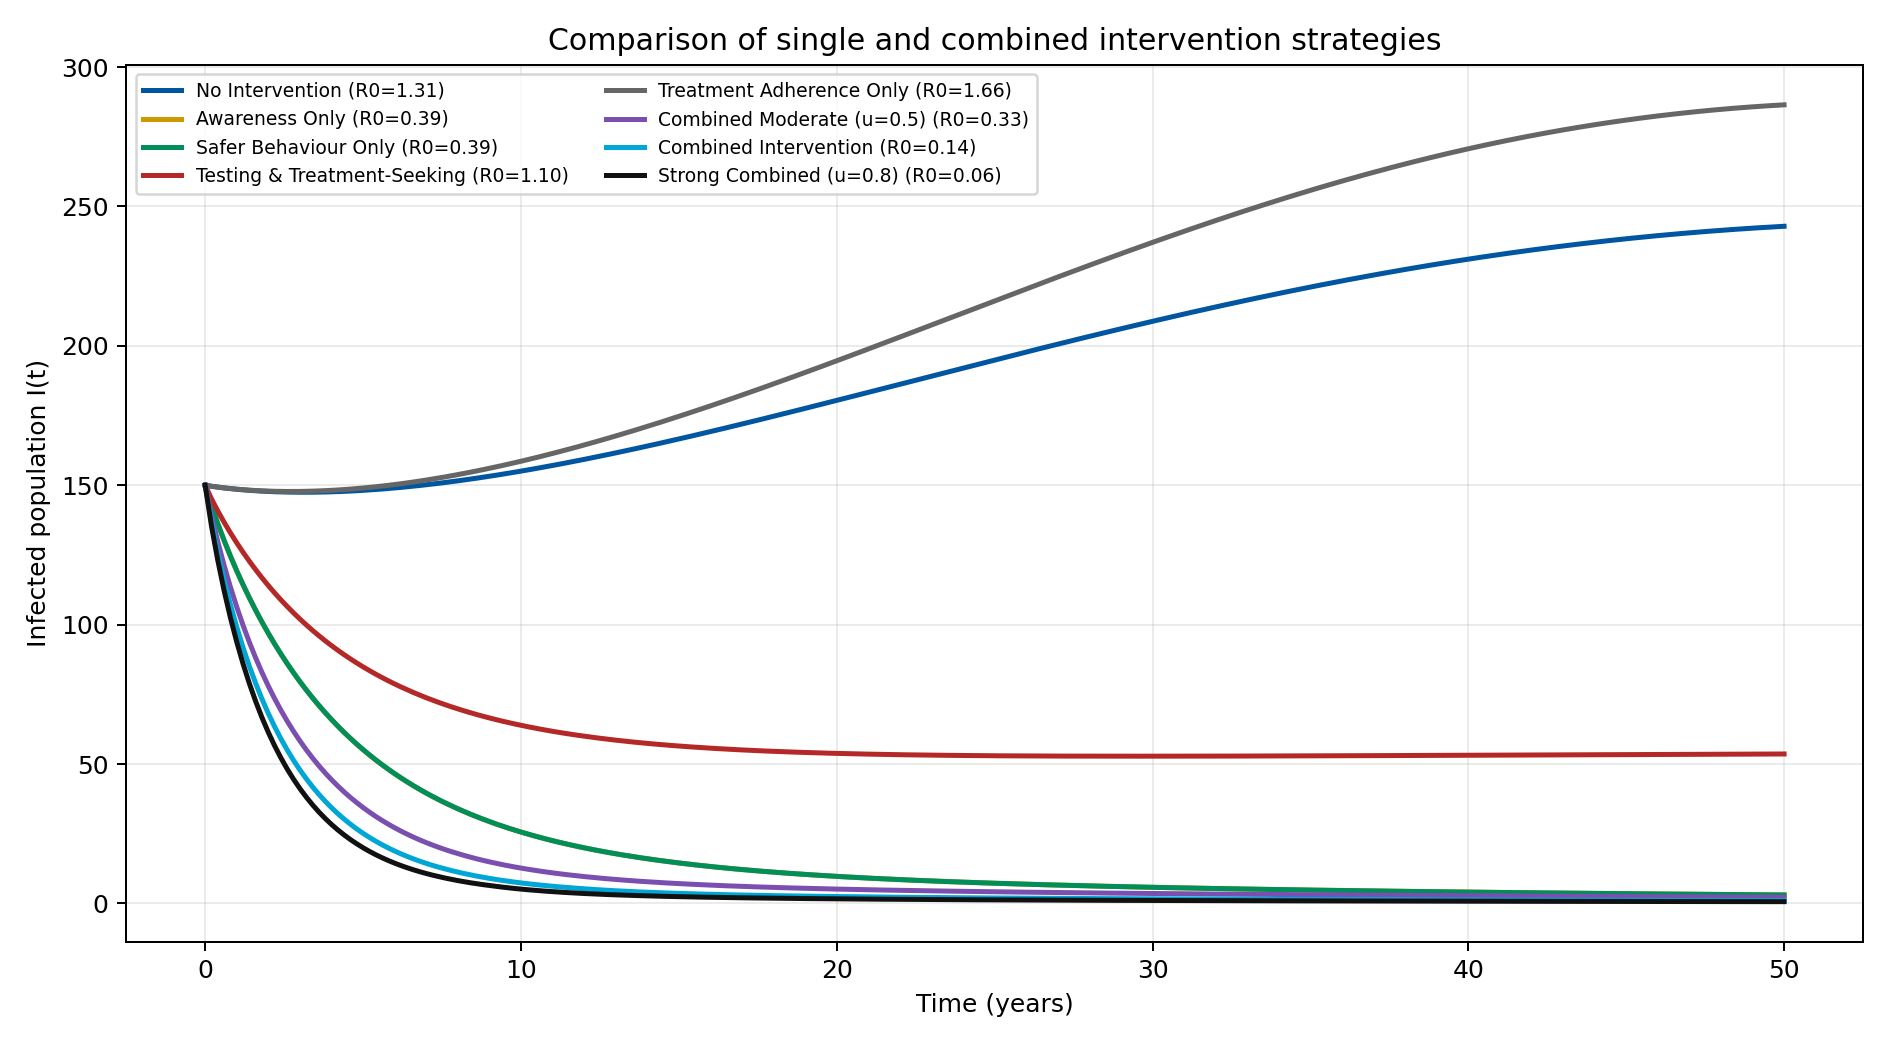
\includegraphics[width=0.95\linewidth]{../thesis/combinedInterventionsChart.png}
      \vspace{0.08cm}
      {\scriptsize\color{Muted}Combined interventions reduce the epidemic burden more strongly than isolated controls.}
    \end{column}
    \begin{column}{0.49\textwidth}
      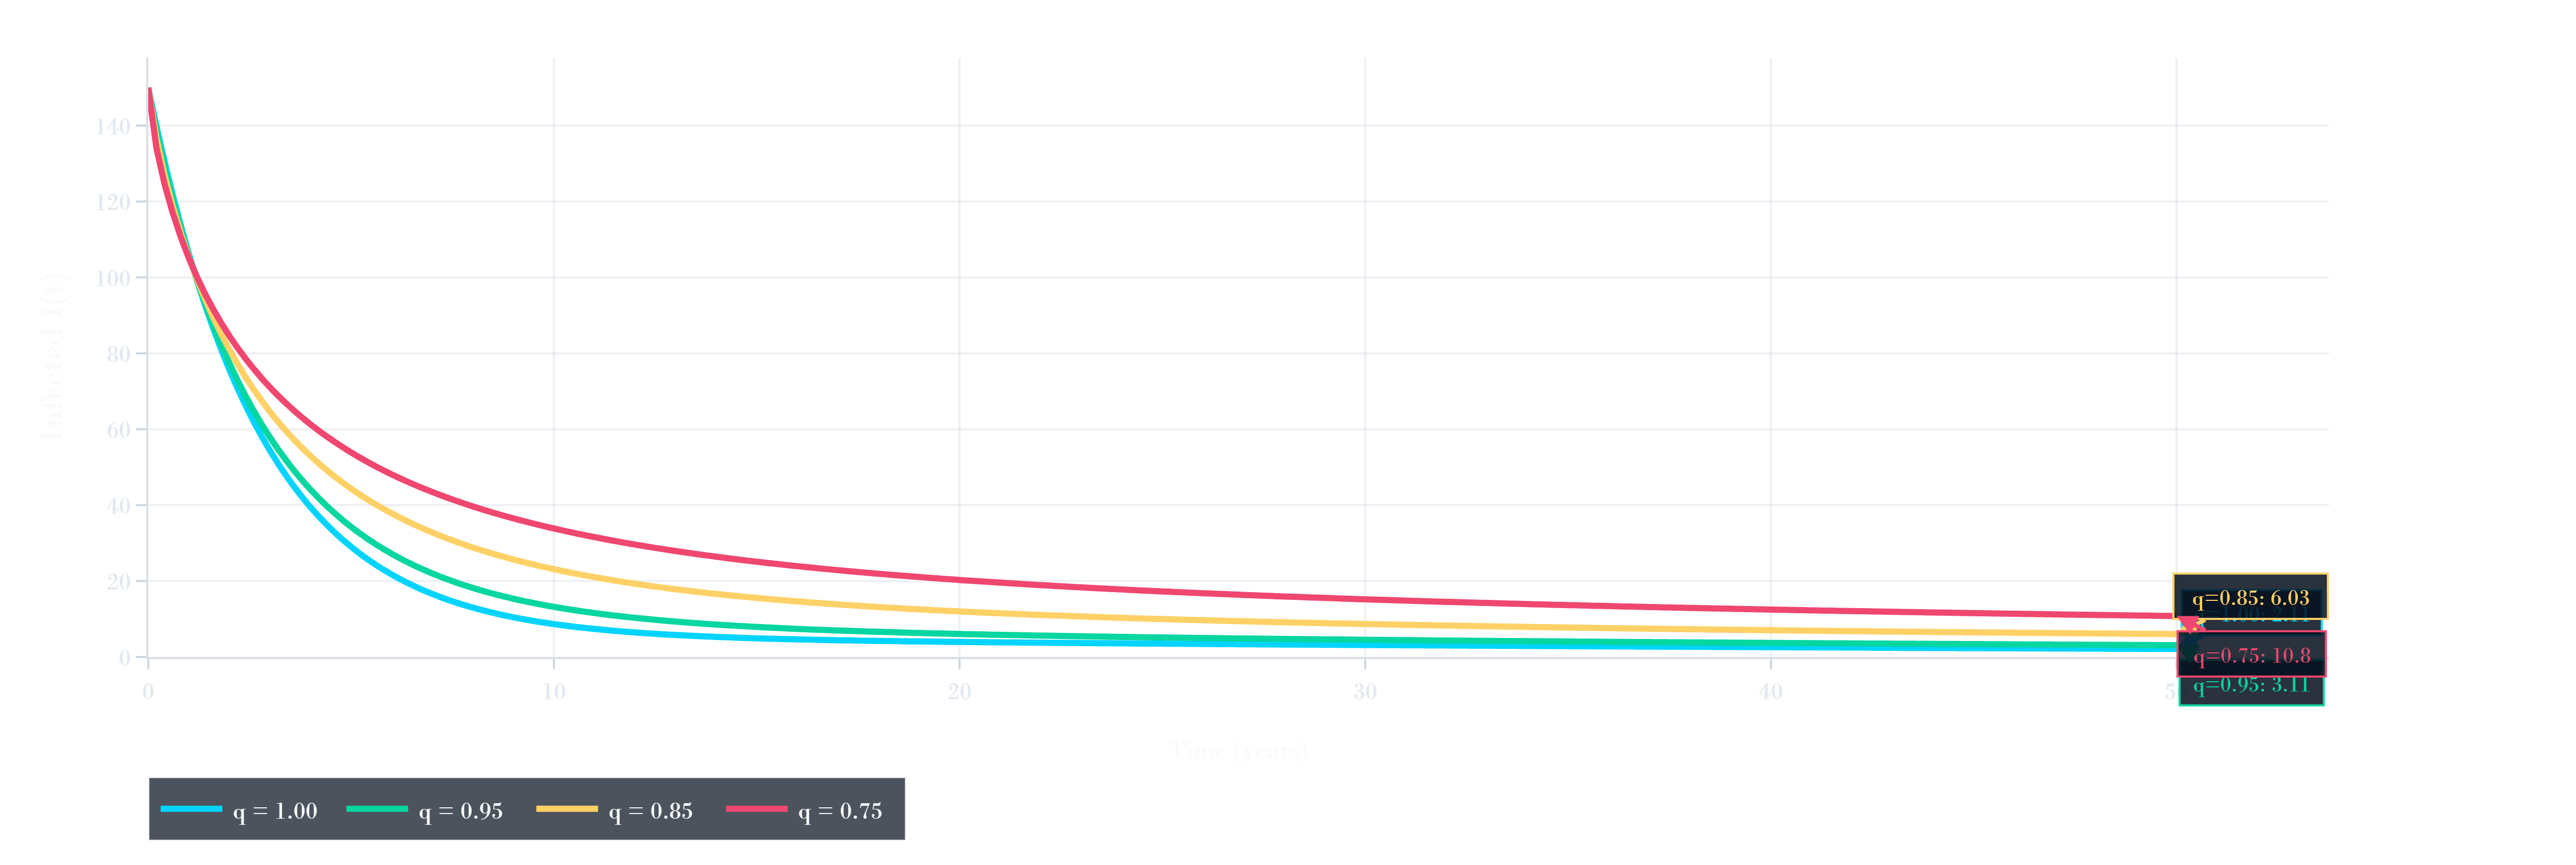
\includegraphics[width=0.95\linewidth]{../thesis/memoryChart.png}
      \vspace{0.08cm}
      {\scriptsize\color{Muted}Changing $q$ shows the visible effect of fractional memory on $I(t)$.}
    \end{column}
  \end{columns}
  \vspace{0.25cm}
  \softbox{SoftBlue}{\textbf{Interpretation:} prevention, testing, treatment uptake, and adherence work best together; lower $q$ values show that past behaviour and treatment history can affect long-term trajectories.}
\end{frame}

% 9
\begin{frame}{Live Demo Plan}
  \begin{columns}[T,onlytextwidth]
    \begin{column}{0.52\textwidth}
      \sectiontag{Demo choreography}
      \begin{enumerate}
        \item Open \texttt{\appurl}.
        \item Show the moving SITA graph: $S(t)$, $I(t)$, $T(t)$, $A(t)$.
        \item Switch from no intervention to combined intervention.
        \item Compare $q=1$ ordinary model with $q<1$ fractional memory.
        \item Open sensitivity and scenario tabs to defend the dashboard evidence.
      \end{enumerate}
    \end{column}
    \begin{column}{0.42\textwidth}
      \sectiontag{What examiners should see}
      \begin{itemize}
        \item The thesis equations are implemented.
        \item Graphs move because the model is being simulated.
        \item The dashboard produces chapter-ready figures and tables.
        \item The work is reproducible and deployed online.
      \end{itemize}
      \vspace{0.25cm}
      \softbox{SoftGold}{\textbf{Key phrase:} ``My main contribution is not only the model, but a working dashboard that allows the model to be explored live.''}
    \end{column}
  \end{columns}
\end{frame}

% 10
\begin{frame}{Conclusion + Recommendations}
  \begin{columns}[T,onlytextwidth]
    \begin{column}{0.5\textwidth}
      \sectiontag{Conclusion}
      \begin{itemize}
        \item A fractional-order SITA HIV model was formulated and implemented.
        \item Social behaviour interventions were incorporated through effective rates.
        \item The dashboard connects theory, computation, scenario analysis, memory effects, and sensitivity results.
      \end{itemize}
    \end{column}
    \begin{column}{0.45\textwidth}
      \sectiontag{Recommendations}
      \begin{itemize}
        \item Continue integrating prevention and treatment-support interventions.
        \item Use Rwanda-specific data in future calibration studies.
        \item Extend the dashboard with uncertainty analysis and richer intervention scenarios.
      \end{itemize}
    \end{column}
  \end{columns}
  \vspace{0.32cm}
  \softbox{SoftBlue}{\textbf{Final message:} the project transforms a fractional HIV model into an interactive Rwanda-aware simulation tool for academic analysis and communication.}
  \vspace{0.18cm}
  \begin{center}
    {\large\bfseries Thank you}\\
    {\small Live dashboard: \texttt{\appurl}}
  \end{center}
\end{frame}

\end{document}
